%(BEGIN_QUESTION)
% Copyright 2011, Tony R. Kuphaldt, released under the Creative Commons Attribution License (v 1.0)
% This means you may do almost anything with this work of mine, so long as you give me proper credit

Koble et «ice cube»-relé til en av utgangene på en PLC, slik at PLC-en kan styre innkobling av reléet. Alle elektriske forbindelser skal gjøres via koblingslist (ingen tvinnede ledninger, krympeskjøter, koblingsmuttere, fjærklemmer eller «krokodilleklemmer»). Programmer denne PLC-en slik at den implementerer en start/stopp-funksjon (latching) for motor. {\it For å sikre at programmet ikke er skrevet på forhånd, vil du først bli bedt om å skissere et korrekt ladderdiagram på papir før du bruker PC.}

Du må koble en «friløpsdiode» parallelt med reléspolen for å hindre fenomenet «induktivt tilbakeslag», som ellers kan skade transistorutgangen på PLC-en. Merk at feil polaritet på dioden gir kortslutning mot PLC-utgangen, så du {\it må} koble den riktig.

Øvelsen tester evnen din til å tolke pinout på et elektromekanisk relé, koble en PLC-utgang riktig til reléspolen, polarisere friløpsdioden korrekt for å beskytte PLC-utgangen, og bruke koblingslist for ryddige forbindelser. Den tester også evnen til å programmere start/stopp-logikk enten med selvholdskontakt eller med latch/retentive spoleinstruksjoner.

$$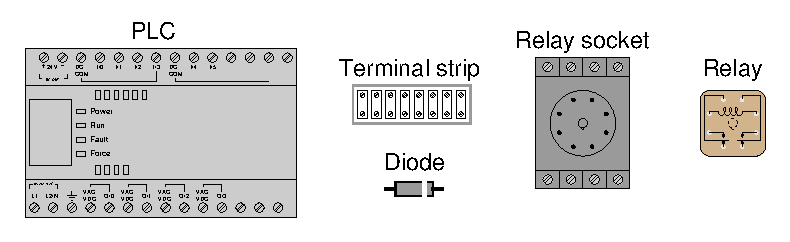
\includegraphics[width=15.5cm]{i00127x01.eps}$$

\vskip 10pt

Følgende komponenter/materialer er tilgjengelige: ulike «ice cube» {\bf reléer} med DC-spoler og tilhørende {\bf sokler}; {\bf koblingslister}; 1N400X likeretter-{\bf dioder}; lengder med {\bf koblingsledning}. Du må selv ha skrutrekkere og multimeter for montering og test ved arbeidsplassen.

\vskip 20pt

\noindent
{\bf «Start»-bryter til inngang}: \underbar{\hskip 20pt} \hskip 30pt {\bf «Stop»-bryter til inngang}: \underbar{\hskip 20pt} \hskip 30pt {\bf Relé til utgang}: \underbar{\hskip 20pt}

\vskip 20pt

\noindent
{\bf PLC-program} (instruktør velger): \hskip 20pt \underbar{\hskip 20pt} Selvholdskontakt \hskip 20pt \underbar{\hskip 20pt} Retentive spoler



\vfil

\underbar{file i00127}
\eject
%(END_QUESTION)





%(BEGIN_ANSWER)


%(END_ANSWER)





%(BEGIN_NOTES)


%INDEX% Mastery exam performance exercise (circuit), drive a relay coil with a PLC output

%(END_NOTES)
